\documentclass{article}

\usepackage{pdfpages}
\usepackage{booktabs}
\usepackage{tabularx}
\usepackage{hyperref}
\usepackage{xcolor}

\title{SE 3XA3: Development Plan\\\textcolor{red}{Snake 2.o}}

\author{Team \# 30, VUA30
		\\ Vaibhav Chadha , chadhav
		\\ Usman Irfan , irfanm7
		\\ Andy Hameed , hameea1
}

\date{}



\begin{document}

\begin{table}[hp]
\caption{Revision History} \label{TblRevisionHistory}
\begin{tabularx}{\textwidth}{llX}
\toprule
\textbf{Date} & \textbf{Developer(s)} & \textbf{Change}\\
\midrule
Sept 25, 2018 & Vaibhav, Usman, Andy & Worked on part 1 to 4\\
Sept 27, 2018 & Vaibhav, Usman, Andy & Worked on part 4 to 8\\
Sept 27, 2018 & Vaibhav & Added the information from the meeting documents to the LaTeX file\\
Sept 28, 2018 & Andy & Proof of concept, Git workflow, Final editing and formatting\\
Sept 28, 2018 & Usman & Updated proof of concept\\
\textcolor{blue}{Oct 12, 2018} & Andy & Made changes according to feedback on development plan and added section on POC demo\\
\textcolor{red}{Dec 2, 2018} & Vaibhav Chadha & Revision one changes to improve the documents quality.\\
\textcolor{red}{Dec 2, 2018} & Usman Irfan & Revision one changes to improve the documents quality.\\
Dec 3, 2018 & Andy & Project Review section completed\\
\bottomrule
\end{tabularx}
\end{table}

\newpage

\maketitle


\section{Team Meeting Plan}
Meetings will be held \textbf{twice a week} at the following times:
\begin{itemize}
\item Mondays 5:30 - 6:30 pm at KTH Computer Labs
\item  Wednesdays 12:30 to 2:00pm at Health science library
\end{itemize}

\subsection{Roles and Agenda}

\textbf{Chair}: Andy Hameed
\begin{itemize}
	\item Responsible for creating the agenda and selecting topics that pertain to all team members
	\item Agenda items will be listed as questions\\
\end{itemize}
\textbf{Notettaker}: Usman Irfan
\begin{itemize}
	\item Responsible for taking meeting minutes
	\item Meeting decisions will be summarized in a statement at the end of the meeting
\end{itemize}
\textbf{Timekeeper}: Vaibhav Chadha
\begin{itemize}
	\item Keeps track of time in case we are spending too much time on one topic
\end{itemize}


\section{Team Communication Plan}
\textcolor{blue}{Main source of communication is Facebook Messenger, it will be used for general inquiries, updates, reminders of team meetings, any links to useful resources and so on. Phone and texting will be used as a backup in case of urgent matters, for example not being able to get in contact with a team member through Messenger.
Aside from these, the team will be using Workflowy to assign small tasks that are promptly due or ones that may not necessarily fit on the \textcolor{red}{Gantt} chart because they are minor - this tool will be used to delegate a small to-do list for each team member.
} 

\section{Team Member Roles}

Vaibhav Chadha:
\begin{itemize}
\item Latex Documentation
\item Analyst - makes sure the requirements of the clients are met through the software
\item \textcolor{red}{Gantt} chart management\\
\end{itemize}
Usman Irfan: 
\begin{itemize}
\item Scribe
\item Technology Research
\item operation manager -ensures project development is running smoothly and software is being developed according to milestones \\
\end{itemize}
Andy Hameed:

\begin{itemize}
\item Final editing
\item latex documentation
\item team leader\\
\end{itemize}

All: 
\begin{itemize}
\item GIT project management
\end{itemize}

\section{Git Workflow Plan}
We will be using the Git Feature Branch Workflow to manage the software development. Using branches, each team member is capable of 
working on different modules or sections of the software at the same time in localized branches, before pushing their changes to the master branch.

The following procedures will be followed:
\begin{itemize}
\item \textcolor{blue}{Vaibhav will be tagging any major milestones for final submission. This makes the submission process consistent. Otherwise, Andy or Usman will agree on one person to tag and submit for final submission.}
\item \textcolor{blue}{Any major changes and submissions, especially those involving a milestone, can be placed in a branch to avoid merging conflicts and overwriting existing work. They can be merged later on upon team agreement.}
\end{itemize}

\section{Proof of Concept Demonstration Plan}
The original project is built using \textcolor{red}{JavaScript}, HTML and CSS in contrast to our development plan using \textcolor{red}{Python} and the Pygame library. Since we are using an OOP language, we will be able to create classes for different components of the snake game such as \textcolor{red}{the snake's body drawn in blocks, and snake's food.} The hardest part of the implementation will be the movement of the snake according to the user's keyboard inputs, and second to that would be the process of expanding the snake once a food item is captured. Besides that, the interface may be difficult to implement in \textcolor{red}{Python using the Pygame library to make it engaging.}\\
	Once our game application has been developed the next part would be to test the project and for that we will be using Pytest, since our backend language is \textcolor{red}{Python} this will help us test all possible functions and \textcolor{red}{functional requirements}. The functions that will be difficult to test would be to see if the snake eats the food, does the food appear at random locations after eaten by the snake and if the snake tries to leave the borders, will the game end. Portability will have to be taken into consideration since the application is being built for \textcolor{red}{different Operating System}. However, it can be compiled and run on any system as long as the necessary files and libraries are download.


\textcolor{blue}{\subsection{POC Demo}
The team will be demonstrating the movement of a snake around the screen using unit blocks for the body of the snake. Lengthening the snake body, scoring and eating the bate will not be demonstrated in the demo. This POC should demonstrate that with the movement of the snake, which is the main component of the game, the team will be able to develop classes to represent other components of the game such as the score, food bate, and lengthening of the snake body.}

\section{Technology}

Coding Language: Python, \textcolor{red}{Pygame} for GUI\\
IDE: IDLE scripting\\
Testing: PyUnit testing\\
Documentation: Doxygen\\

\section{Coding Style}

We will be using the \href{https://github.com/google/styleguide/blob/gh-pages/pyguide.md}{Google Python Style Guide}
for our coding style. It encompasses all the necessary naming conventions and standards required for the project development.

\section{Project Schedule}
Please see the following pages for the project schedule in the form of a \textcolor{red}{Gantt Chart}.

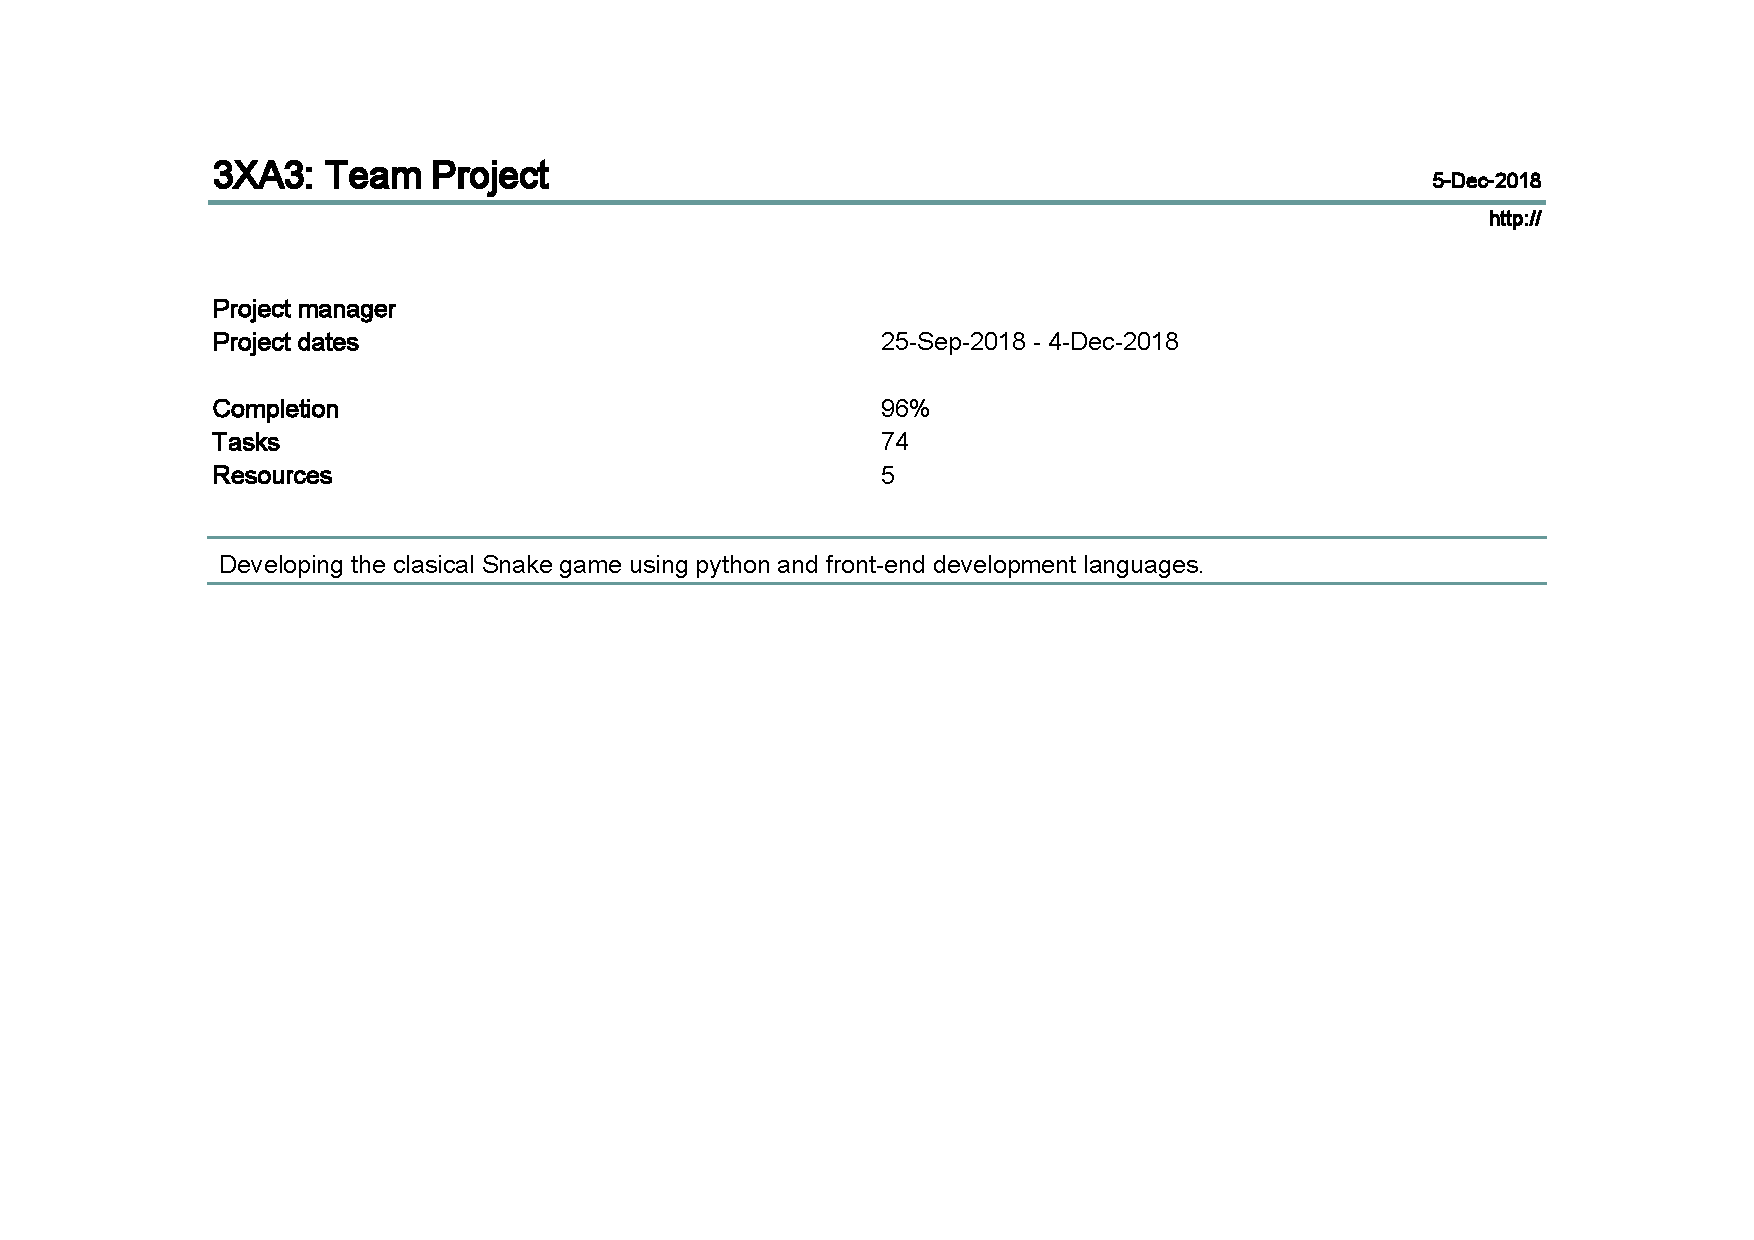
\includepdf[page=-]{DevPlan_ExpandedGantt}

\section{Project Review}

The Snake 2.o project ultimately produced three quantifiable assets to the original Snake Game project. The change in game environment from an online playable version to a desktop version allowed for portability and non restrictive playing conditions after the initial download. Rearranging the game buttons and features in a new layout along with a complementary color scheme improved the overall aesthetics of the game, creating a positive and pleasant gameplay experience. In addition, the themes and difficulty modes added to the game added a twist to the orignal game, giving the reimplementation a unique characteristics that is typically missing from remakes of the game. 

The project objectives that were set out in the beginning have been acheived. Future plans for the project include the following changes and additions:
\begin{itemize}
\item Additional theme options besides the existing dark, regular and random themes
\item Smoother snake movements and snake visual representation
\item harder modes and additional levels with unique elements drawn from peer feedback
\item game window resizing ability
\end{itemize}

Note that this is a brief list of some of the ideas and plans for future implementation objectives and tasks. However, it is not an exhaustive list and will continue to change as the project progresses.

\end{document}